\documentclass{beamer}
\graphicspath{ {../../instances/} }

%Information to be included in the title page:
\title{MAPF project: first steps}
\author{Andrés Córdova and Aleksandra Khatova}
\institute{Unversity of Potsdam}
\date{2022}

\AtBeginSection[]
{
  \begin{frame}
    \frametitle{Table of Contents}
    \tableofcontents[currentsection]
  \end{frame}
}

\begin{document}

\frame{\titlepage}

\begin{frame}
\frametitle{General approach}
\begin{itemize} 
\item<1-> Create a test instance
\item<2-> Break a test instance into many similar, one for each robot
\item<3-> Use asprilo to create plans for each robot separately
\item<4-> Merge these plans and resolve conflicts
\end{itemize} 
\end{frame}

\begin{frame}
\frametitle{Test instance}
\centering
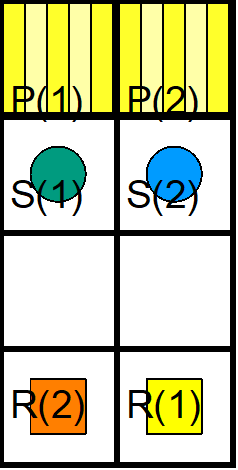
\includegraphics[scale=0.2]{x3y2r1s2p2.png}
\end{frame}

\begin{frame}
\frametitle{Separate test instances for each robot}
\centering
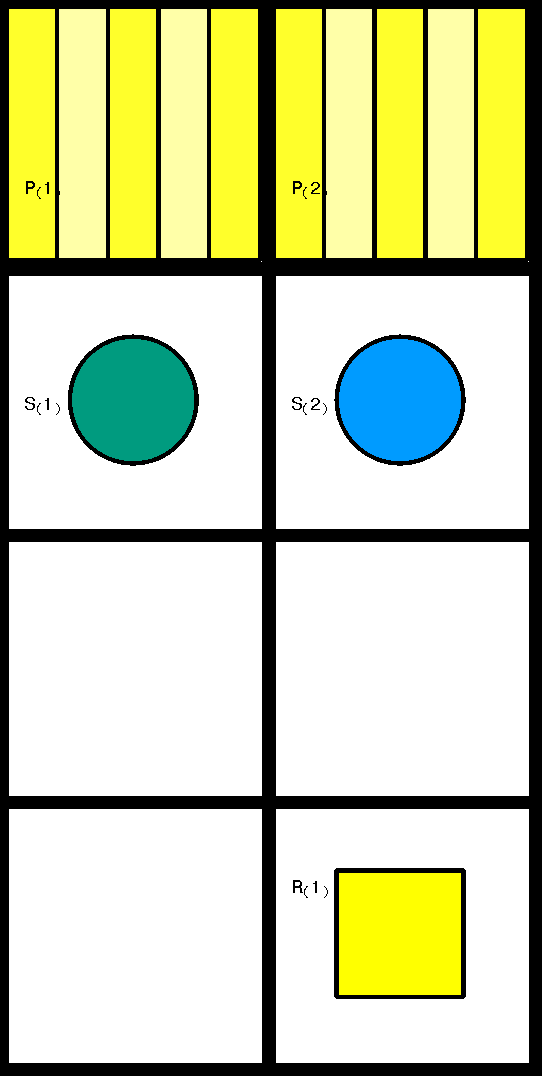
\includegraphics[scale=0.2]{x3y2r1s2p2_1.png}
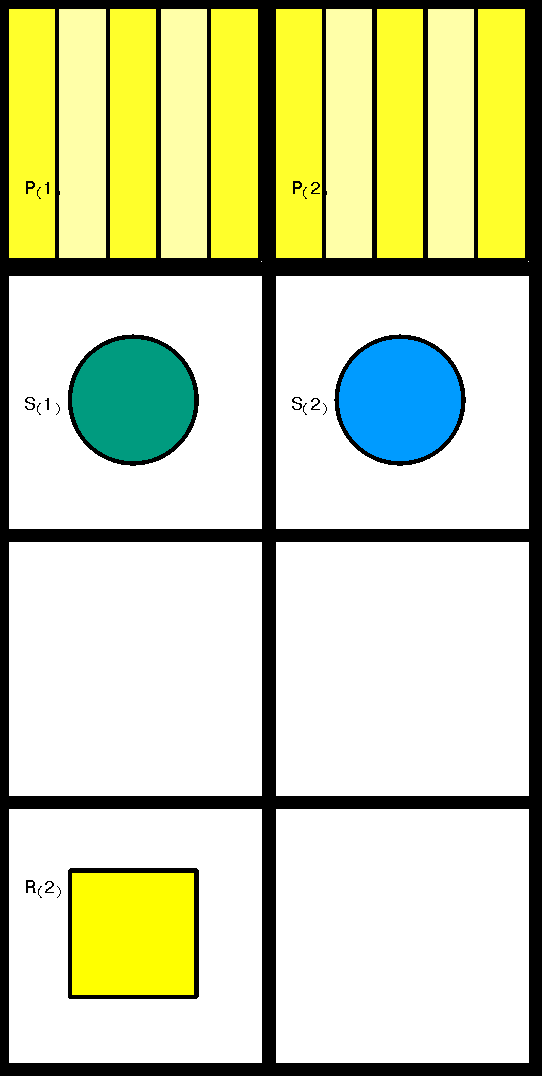
\includegraphics[scale=0.2]{x3y2r1s2p2_2.png}
\end{frame}

\begin{frame}
\frametitle{Use asprilo to create plans}
\centering
See visualizer
\end{frame}

\begin{frame}
\frametitle{Use asprilo to create plans}
\centering
Conflict: edge collision
\end{frame}

\begin{frame}
\frametitle{Merging strategy for edge collision conflicts}
\begin{itemize} 
\item<1-> Copy moves that don't cause conflicts
\item<2-> If collision detected:
\begin{enumerate}
\item<3-> Move in the direction perpendicular to the direction of the collision
\item<4-> Move parallel to the move which caused the collision
\item<5-> Move back to your initial plan
\end{enumerate}
\item<6-> Each collision resolution adds 2 moves to the plan
\end{itemize} 
\end{frame}

\begin{frame}
\frametitle{Result of merging}
\centering
See visualizer
\end{frame}

\begin{frame}
\frametitle{Use asprilo to create plans}
\centering
Conflict resolved
\end{frame}

\begin{frame}
\frametitle{Plans for further work}
\begin{itemize} 
\item<1-> Automate whatever is possible to automate
\item<2-> Define other types of conflicts
\item<3-> Try other strategies, starting with simpler ones
\end{itemize} 
\end{frame}

\end{document}